% Chapter 1

\chapter{Introducción} % Main chapter title

\label{Chap:Intro} % For referencing the chapter elsewhere, use \ref{Intr} 

%----------------------------------------------------------------------------------------

% Define some commands to keep the formatting separted from the content 
\newcommand{\keyword}[1]{\textbf{#1}}
\newcommand{\tabhead}[1]{\textbf{#1}}
\newcommand{\code}[1]{\texttt{#1}}
\newcommand{\file}[1]{\texttt{\bfseries#1}}
\newcommand{\option}[1]{\texttt{\itshape#1}}

%----------------------------------------------------------------------------------------

\section{Preliminares}
En este documento de tesis se presenta la implementación de un sistema de navegación RTK (Real-Time Kinematics\footnotemark) con el apoyo de un software dedicado a navegación en una computadora portátil de bajo costo, basándose en el trabajo de \cite{takasu2009development}.

\footnotetext{Sistema de Navegación en Tiempo Real por sus siglas en inglés.}

\section{Importancia del tema}
La humanidad ha estado interesada en obtener información acerca del contexto en el que interactúa para poder utilizarlo a su favor. \\

A través del tiempo, se ha aumentado la certeza de los datos contenidos, por ejemplo, en un mapa, debido al aumento de la precisión de las herramientas de medición utilizadas. Un ejemplo de dichas herramientas son las computadoras, sensores y actuadores, así como de algoritmos que permiten filtrar errores aleatorios. \\

Mediante el uso de un sistema de navegación en tiempo real (RTK), se tiene como finalidad obtener la información de navegación de un vehículo de forma que este sistema pueda aportar datos confiables medibles en pocos decímetros para apoyar en el control de posicionamiento del mismo.

\section{Planteamiento del Problema}
A pesar del avance de la tecnología en las herramientas de medición, aún persisten algunos errores en la precisión, que de forma práctica, afectan al implementar sistemas basados en ellos. \\

\begin{figure}[H]
\centering
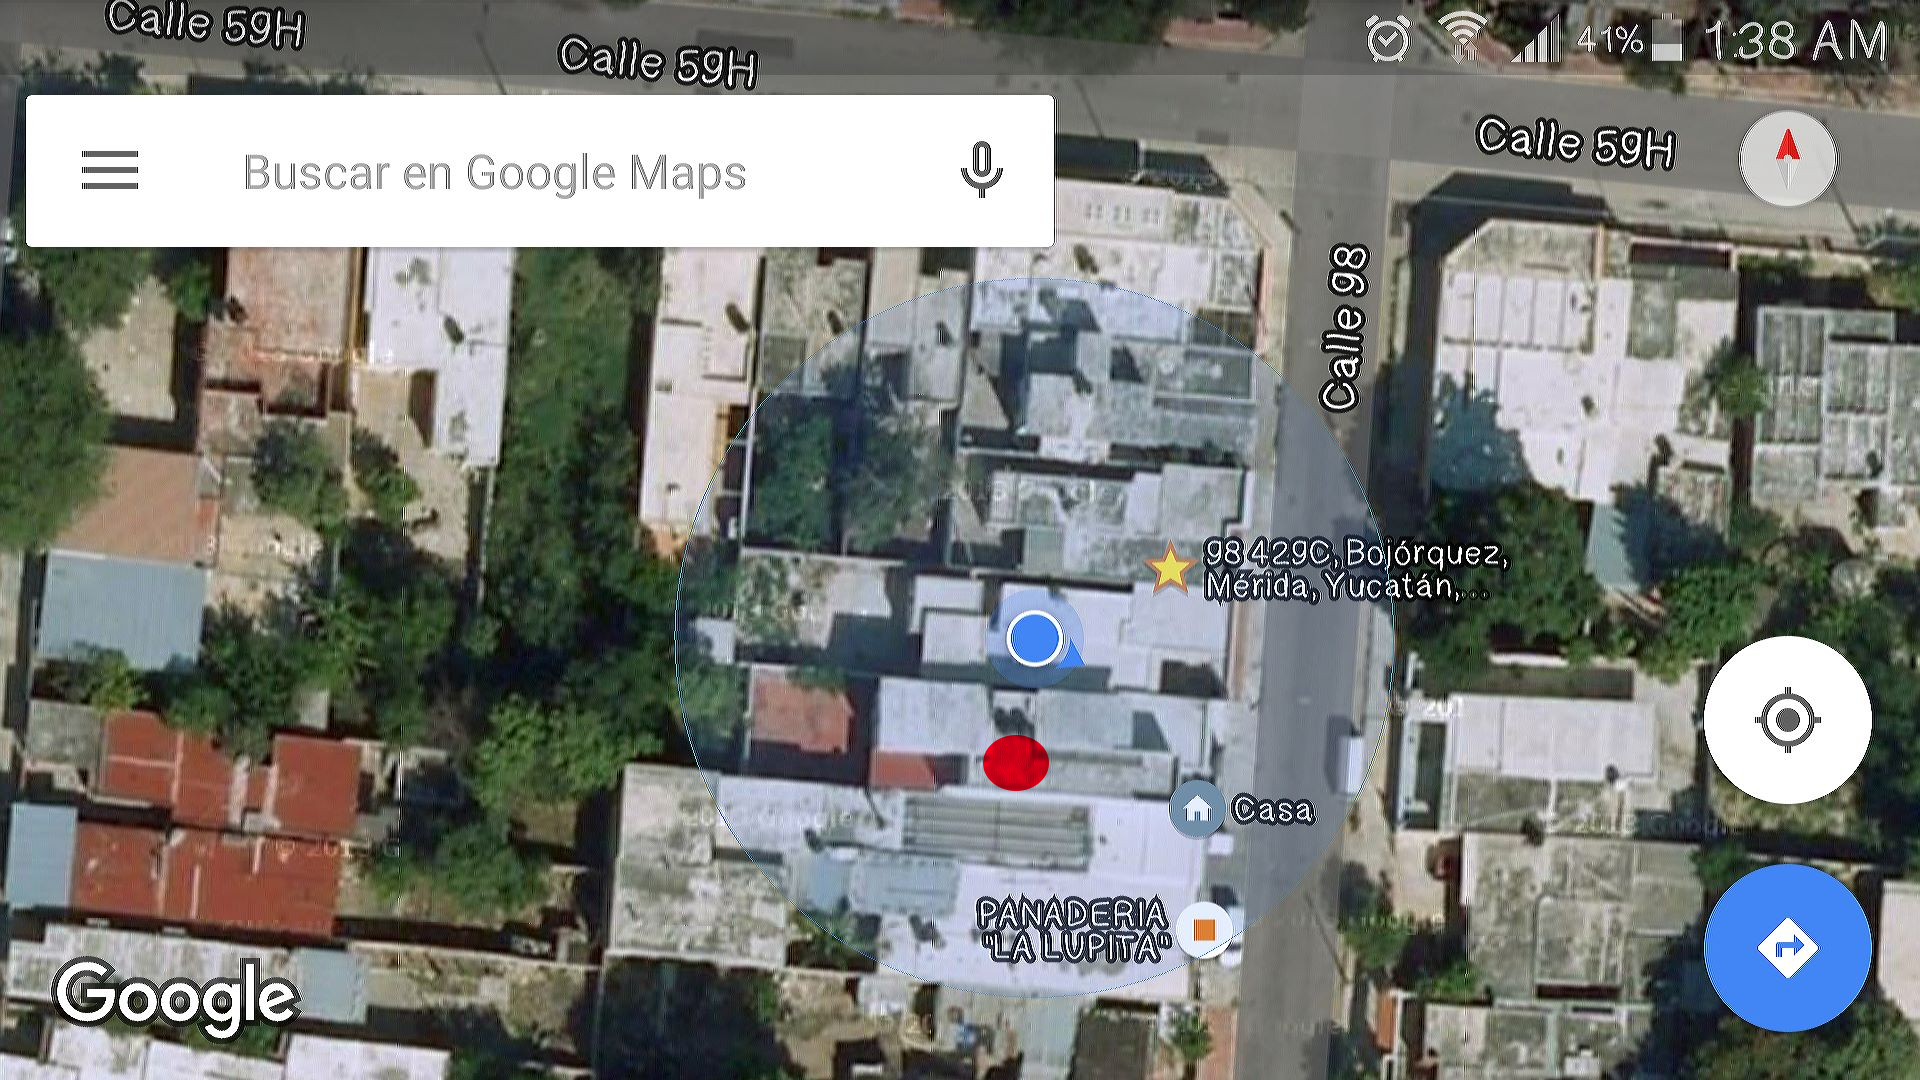
\includegraphics[scale=0.2]{Figures/Pred}
\caption[Posición de celular en mapa.]{Posición aproximada de la ubicación de un celular en un mapa de Google Maps.}
\label{fig:Prec}
\end{figure}

En una planeación de ruta de un sistema de navegación autónomo, una incertidumbre de $n$ metros a la redonda converge en una inexactitud significativa del sistema. El dispositivo puede encontrarse dentro de cualquier punto de la circunferencia de $2n$ metros de diámetro. Como se puede observar en la figura~\ref{fig:Prec}, todo el círculo azul denota la posición aproximada de un dispositivo celular con GPS, y en donde la pequeña elipse roja muestra la posición real en dicho mapa. La circunferencia del círculo azul abarca prácticamente la mitad de una manzana, haciendo notorio un problema de impracticidad al intentar implementar un sistema de posicionamiento de, por ejemplo, un automóvil autónomo.

\section{Trabajos previos}
En la tesis de \cite{de2011diseno}, se usa un sistema GPS (Global Positioning System\footnotemark) para apoyar en la logística de distribución de farmacéuticos, como control de rutas, tiempos y seguridad, mencionando ante todo la capacidad de poder obtener los datos de localización y tiempo, además de la velocidad de desplazamiento de un vehículo. Sin embargo, de acuerdo al artículo de \cite{mendoza2004recomendaciones}, donde se propone una actualización del ancho de carriles carreteros a una amplitud adecuada máxima de 3.6 m, dado que un GPS mide su incertidumbre en una escala de metros, podría indicar que el vehículo se encuentra fuera de la cinta asfáltica o circulando en una vía contraria. Por tanto, se hace importante que un sistema tenga un menor grado de incertidumbre al ofrecido de forma estándar con GPS, como el Real-Time Kinematics, medido en pocos decímetros de error. \\

\footnotetext{Sistema de Posicionamiento Global, por sus siglas en inglés.}

También, la tesis escrita por \cite{ronnback2000developement}, menciona la implementación de un sistema de navegación inercial INS/GPS para un UAV (Unmanned Aerial Vehicle\footnotemark). Entre los datos a destacar, la posición de este sistema es estimada con un error de 2 m con un 95\% de confianza, además de otros datos para asistir al vuelo como velocidad y su altitud. Una incertidumbre de 2 m hace inviable que un drone (vehículo aéreo no tripulado) pudiese mantenerse cuando se le requiere que esté estático, por ejemplo, en fotografía aérea.\\

\footnotetext{Vehículo Aéreo No Tripulado, por sus siglas en inglés.}

Revisando el artículo de \cite{maldonado2010controlador}, los autores afirman que las coordenadas recibidas de un dispositivo GPS solamente son usadas como aproximación a la posición del vehículo, y nunca como un dato sólido que sirviese al computar datos, dada la exactitud mínima de 10 metros. Sin embargo, mencionan limitantes tales como el peso total de la carga del UAV y el consumo de energía causado por la integración de todos los demás sensores, de donde el GPS aporta entonces una cantidad mínima de información y utilidad en general. Sería ideal que el sistema de posicionamiento aportara información más precisa y que aporte a las observaciones realizadas con el vehículo de forma general.\\


\subsection{Propuesta}
Dado que en los trabajos previos se presentan algunos inconvenientes con la presición del sistema de navegación inercial de los dispositivos debido a la naturaleza del sensor GPS común utilizado, se propone la realización de un sistema de navegación que utilice una aplicación de cómputo denominada RTKLIB, que nominalmente reduce el error a una escala medible en centímetros a partir de dos señales de GPS, en un sistema portátil de arquitectura ARM (Advanced RISC Machine), ampliando las posibilidades de aprovechamiento de los datos.

\section{Hipótesis}
Mediante corrección diferencial de tipo Real-Time Kinematics, se puede reducir la incertidumbre de un equipo GPS a niveles de escasos decímetros.

\section{Objetivo}
\subsection{General}
El objetivo general de este trabajo es el diseño y la implementación de un sistema de navegación capaz de conocer su ubicación en un entorno geográfico con una alta precisión para apoyar en proyectos que requieran de dicha información, utilizando dispositivos pequeños y portátiles.

\subsection{Objetivos específicos}
\begin{itemize}
	\item Configurar los GPS en dos estaciones: una móvil y una base.
    \item Configurar la transferencia de datos entre estaciones en UHF (Ultra-High Frequency\footnotemark).
    \item Acondicionamiento de una microcomputadora BeagleBone con sus respectivos periféricos de apoyo.
    \item Programación de una biblioteca que controle los periféricos a través de la microcomputadora.
    \item Integración de módulos.
	\item Evaluación de los datos obtenidos.   
\end{itemize}

\footnotetext{Ultra Alta Frecuencia, por sus siglas en inglés.}

\section{Publicaciones}

Los avances de este proyecto fueron publicados en las memorias en extenso del Encuentro Universitario de Sistemas Computacionales - EUSICS 2016.

\section{Descripción del documento}

El presente trabajo se divide en las siguientes secciones: 

\begin{itemize}
\item \textbf{Introducción:} Se describen tanto la importancia del tema, los problemas a resolver, estado del arte, y una lista de objetivos a seguir durante el desarrollo del tema.\\
\item \textbf{Marco Teórico:} En este apartado se sientan las bases de funcionamiento de los dispositivos a utilizar, así como información útil acerca de los mismos. Se da una descripción general tanto del hardware como del software utilizado.\\
\item \textbf{Diseño del Hardware y Software:} En esta sección se enlistan diversos recursos implementados en el trabajo, tanto de software como de hardware. Se da una descripción de cada uno y el aporte que tienen a la estructura final durante el funcionamiento.\\
\item \textbf{Diseño del Experimento:} Se describen las condiciones a las que será sometido el prototipo para indicar un adecuado funcionamiento de acuerdo a los objetivos listados en la introducción.\\
\item \textbf{Análisis de Resultados:} Se realiza una evaluación de los resultados obtenidos durante la ejecución de la rutina experimental. Se enfatizan diferencias de los distintos modos de funcionamiento y su impacto en el rendimiento del sistema.\\
\item \textbf{Conclusiones:} En forma de síntesis, se da un resumen de los resultados obtenidos de acuerdo al modo de funcionamiento, las observaciones  y el rendimiento en general del sistema.\\
\end{itemize}

Además, al final se añade una sección de anexos en donde se adjuntan guías de configuración o programación de distintos dispositivos de hardware o de software necesarios para la reproducción del proyecto.\\

%En el capítulo~\ref{Chap:Marco}, se expone la teoría que se encuentra detrás de la metodología implementada en el proyecto de tesis, partiendo desde la definición de un sistema GPS, pasando por su modo de funcionamiento y las principales causas de error en sus mediciones. También, se presenta una breve descripción del funcionamiento de una comunicación inalámbrica, del software y del hardware utilizado.